\documentclass[a4paper,10pt]{article}
\usepackage{fontspec}
\usepackage{setspace}
\usepackage{booktabs}
\usepackage{amsmath}
\usepackage{cancel}
\usepackage{graphicx}
\usepackage{biblatex}
\usepackage{float}
\usepackage{tabularx}
\usepackage{booktabs}

\setmainfont{arial}
\setstretch{1.15}
\addbibresource{refs.bib}

\title{Segmentation and Feature Extraction}
\author{Arif Suganda\\
        Tadulako University\\
        \texttt{f5522530002@untad.ac.id}
}

\begin{document}
\maketitle

\section{Edge Detection}
Edge detection is a process to identify the boundaries within an image by using the feature changes within an image.
These boundaries refers to object in the images such as items, shadows, or changes in the object orientation.
The basic method in edge detection is to observe a sudden brightness changes in a digital image, 
but depending on the image condition, precision, cost or speed there several different algorithm that can be used.

\subsection{Roberts}
The roberts operator is one of the oldest and the simplest egde detection methods.
It use a $2 \times 2$ kernel to compute the gradient of each pixel neighborhood by calculating the differece between diagonally adjecent pixels.
Because it only use small kernel it is extremely fast and ``cheap'', but very sensitive to noise.

The implementation of roberts algorithm is using the grayscalled version of Figure~\ref*{fig:image}.

\begin{figure}[H]
    \centering
    
\includegraphics[width=0.6\textwidth]{image.png} 
    \caption{Original image}\label{fig:image}
\end{figure}

The codes for roberts implementation are:

\begin{verbatim}
import cv2
import numpy as np
import matplotlib.pyplot as plt

img = cv2.imread('image.png', cv2.IMREAD_COLOR)
img = cv2.cvtColor(img, cv2.COLOR_BGR2GRAY)

kernel_roberts_x = np.array([[1, 0], [0, -1]])
kernel_roberts_y = np.array([[0, 1], [-1, 0]])
roberts_x = cv2.filter2D(img, -1, kernel_roberts_x)
roberts_y = cv2.filter2D(img, -1, kernel_roberts_y)
roberts_combined = cv2.addWeighted(
        roberts_x, 0.5, roberts_y, 0.5, 0)

fig, ax = plt.subplots(1, 2, figsize=(10, 5))
ax[0].imshow(img, cmap='gray')
ax[0].set_title('Original',)
ax[0].axis('off')
ax[1].imshow(roberts_combined,cmap='gray')
ax[1].set_title('Roberts')
ax[1].axis('off')
plt.tight_layout()
plt.show()
\end{verbatim}

Result:

\begin{figure}[H]
    \centering
    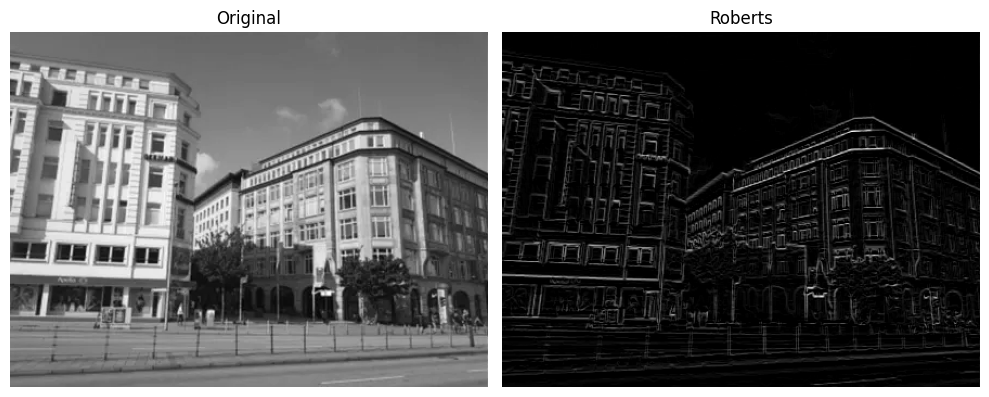
\includegraphics[width=1\textwidth]{roberts.png} 
    \caption{Roberts}\label{fig:roberts}
\end{figure}

\subsection{Prewitt}
The prewitt operators uses two masks of $3 \times 3$ kernels for horizontal and vertical changes, then average the pixel differences which provides a bit of smooting effect.
Because it use a bigger kernel it is better at detecting edges than roberts and slighly less sensitive to noise.
But the edges it produce can appears to be a bit blurry or thick.

The codes for the prewitt implementation using the same import as roberts are:
\begin{verbatim}
kernel_prewitt_x = np.array([[1, 0, -1], [1, 0, -1], [1, 0, -1]])
kernel_prewitt_y = np.array([[1, 1, 1], [0, 0, 0], [-1, -1, -1]])
prewitt_x = cv2.filter2D(img, -1, kernel_prewitt_x)
prewitt_y = cv2.filter2D(img, -1, kernel_prewitt_y)
prewitt_combined = cv2.addWeighted(
        prewitt_x, 0.5, prewitt_y, 0.5, 0)

fig, ax = plt.subplots(1, 2, figsize=(10, 5))
ax[0].imshow(img, cmap='gray')
ax[0].set_title('Original',)
ax[0].axis('off')
ax[1].imshow(prewitt_combined,cmap='gray')
ax[1].set_title('Prewitt')
ax[1].axis('off')
plt.tight_layout()
plt.show()
\end{verbatim}

The result and comparison from Figure~\ref*{fig:image} can be seen below:
\begin{figure}[H]
    \centering
    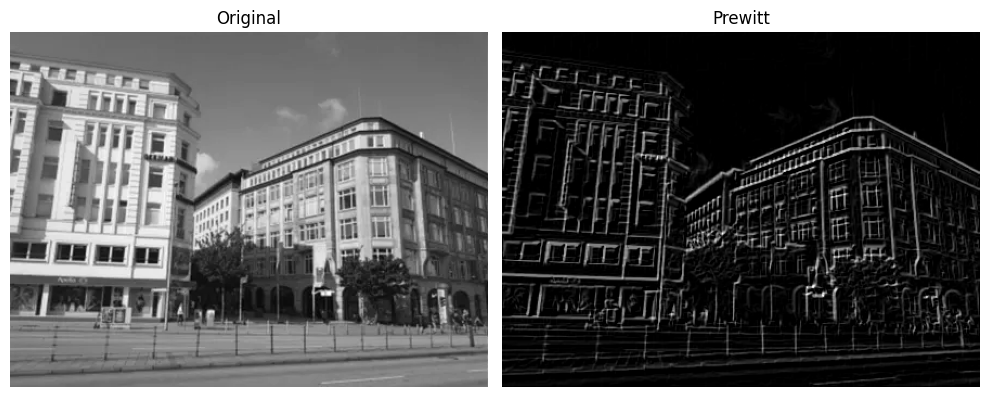
\includegraphics[width=1\textwidth]{prewitt.png} 
    \caption{Prewitt}\label{fig:prewitt}
\end{figure}

\subsection{Sobel}
The sobel operator are similar to prewitt using $3 \times 3$ kernel but adds a weighting factor,
which gives more importance (weight) for a pixel at the center of the mask.
The weighting provides a superior noise suppression compare to prewitter while still being fast.
Similarly to prewitt it can produce thick edges that aren't perfectly precise.

The codes for the sobel implementation using the same import as roberts are:
\begin{verbatim}
sobelx = cv2.Sobel(img, cv2.CV_64F, 1, 0, ksize=3)
sobely = cv2.Sobel(img, cv2.CV_64F, 0, 1, ksize=3)
sobel_combined = cv2.magnitude(sobelx, sobely)

fig, ax = plt.subplots(1, 2, figsize=(10, 5))
ax[0].imshow(img, cmap='gray')
ax[0].set_title('Original',)
ax[0].axis('off')
ax[1].imshow(sobel_combined,cmap='gray')
ax[1].set_title('Sobel')
ax[1].axis('off')
plt.tight_layout()
plt.show()
\end{verbatim}

The result and comparison from Figure~\ref*{fig:image} can be seen below:
\begin{figure}[H]
    \centering
    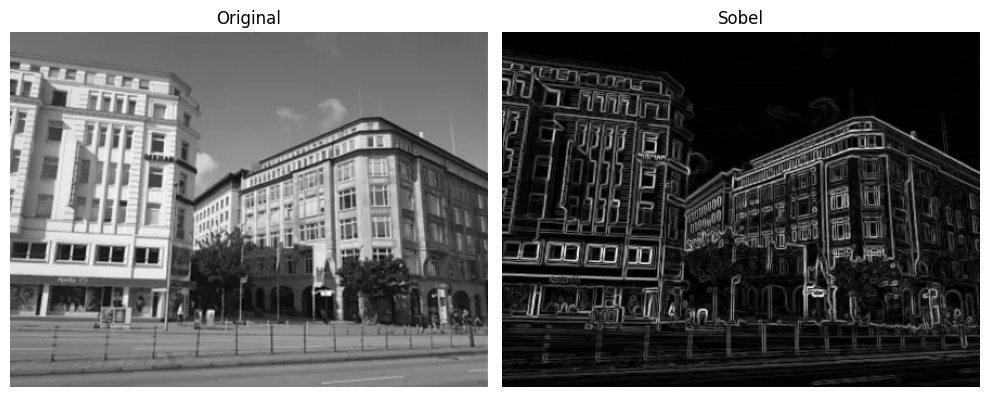
\includegraphics[width=1\textwidth]{sobel.png} 
    \caption{Sobel}\label{fig:sobel}
\end{figure}

\subsection{Canny}
The canny operator unlike the previous operator is a multi-stage algorithm designed for optimal edge detector.
The 5 steps of Canny are:
\begin{enumerate}
        \item Gaussian Blur: Removes noise so the computer doesn't find ``fake'' edges.
        \item Gradient Calculation: Finds the intensity changes (often using Sobel).
        \item Non-Maximum Suppression: Thins the edges down to a single pixel width by ``shaving off'' pixels that aren't the local maximum.
        \item Double Thresholding: Identifies ``strong'' pixels, ``weak'' pixels, and ``irrelevant'' pixels.
        \item Edge Tracking by Hysteresis: Suppresses weak pixels unless they are connected to a strong pixel (ensuring the lines are continuous).
\end{enumerate}


The codes for the canny implementation using the same import as roberts are:
\begin{verbatim}
canny_edges = cv2.Canny(img, 120, 120)

fig, ax = plt.subplots(1, 2, figsize=(10, 5))
ax[0].imshow(img, cmap='gray')
ax[0].set_title('Original',)
ax[0].axis('off')
ax[1].imshow(canny_edges,cmap='gray')
ax[1].set_title('Canny')
ax[1].axis('off')
plt.tight_layout()
plt.show()
\end{verbatim}

The result and comparison from Figure~\ref*{fig:image} can be seen below:
\begin{figure}[H]
    \centering
    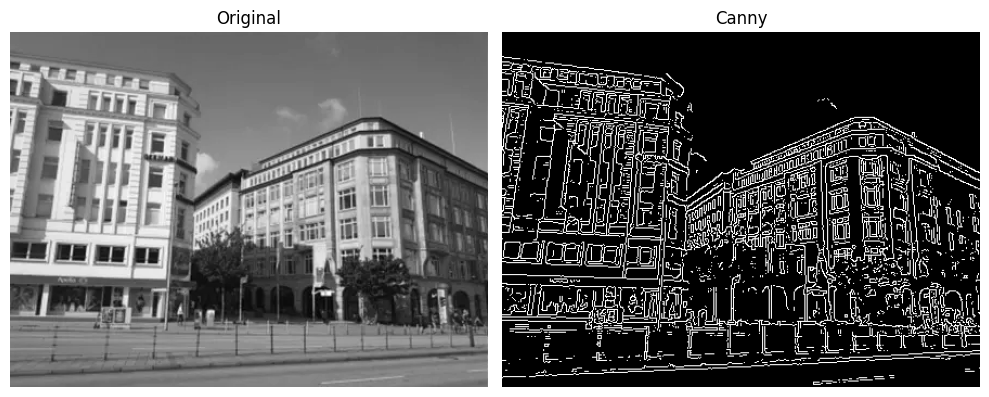
\includegraphics[width=1\textwidth]{canny.png} 
    \caption{Canny}\label{fig:canny}
\end{figure}

\subsection{Comparison}
Using theory and implementation above we can conclude the comparison of each algorithm into Table~\ref*{tab:edge_detection_comparison}

\begin{table}[H]
    \centering
    \footnotesize
    \caption{Comparative Analysis of Edge Detection Algorithms}\label{tab:edge_detection_comparison}
    \begin{tabular}{@{}lccccc@{}}
        \toprule
        \textbf{Algorithm} & \textbf{Complexity} & \textbf{Speed} & \textbf{Noise Sensitivity} & \textbf{Edge Thickness} & \textbf{Accuracy} \\
        \midrule
        \textbf{Roberts}   & Very Low & Fastest & High & Thin & Poor \\
        \textbf{Prewitt}   & Low & Fast & Moderate & Thick & Fair \\
        \textbf{Sobel}     & Low & Fast & Low & Thick & Good \\
        \textbf{Canny}     & High & Slower & Very Low & Thin (1-px) & Excellent \\
        \bottomrule
    \end{tabular}
\end{table}

The implementation also shows that the depths and shadows from the original image is show better in the sobel operator than other operators.
The canny operator edge detection unlike other operator converts the edges into a lines and unlike others it has no blur.
The roberts has the least blur compared to prewitt and sobel and preserve the depth quite well.
The prewitt appears the worst with highest contrast and preserve the edge worst in brighter color.

\section{Segmentation}
\subsection{Tresholding Global}
Global thresholding use a single value for the whole image

Code:
\begin{verbatim}
ret, global_thresh = cv2.threshold(img, 
    127, 255, cv2.THRESH_BINARY + cv2.THRESH_OTSU)

plt.imshow(global_thresh, cmap='gray')
plt.title('Global')
plt.axis('off')
plt.show()
\end{verbatim}

Result can be shown on Figure~\ref*{fig:global_threshold}

\begin{figure}[H]
    \centering
    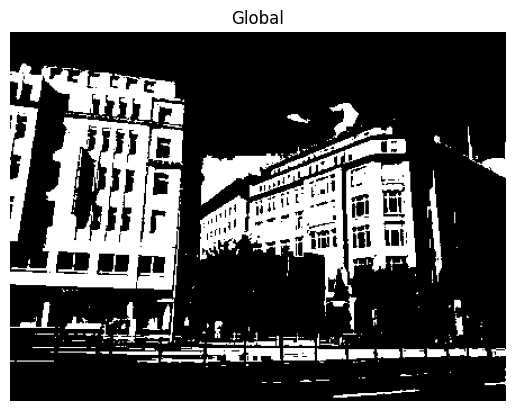
\includegraphics[width=1\textwidth]{global_threshold.png} 
    \caption{Global threshold}\label{fig:global_threshold}
\end{figure}

\subsection{Adaptive Tresholding}
Adaptive thresholding calculates different thresholds for different region in the image which is useful for uneven lightning.

Code:
\begin{verbatim}
adaptive_thresh = cv2.adaptiveThreshold(
    img, 255, cv2.ADAPTIVE_THRESH_GAUSSIAN_C, 
    cv2.THRESH_BINARY, 11, 2)

plt.imshow(adaptive_thresh, cmap='gray')
plt.title('Adaptive')
plt.axis('off')
plt.show()
\end{verbatim}

Result can be shown on Figure~\ref*{fig:adaptive_threshold}

\begin{figure}[H]
    \centering
    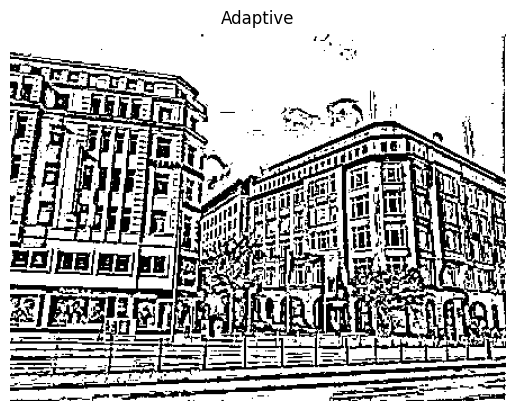
\includegraphics[width=1\textwidth]{adaptive_threshold.png} 
    \caption{Adaptive threshold}\label{fig:adaptive_threshold}
\end{figure}
\subsection{K-Means Clustering}
K-means segmented an image by grouping pixels with similar color. 
Unlike thresholding which can only works on greyscale image, K-means works on color images and can handle more than two segments.

Code:
\begin{verbatim}
from sklearn.cluster import KMeans
import matplotlib.pyplot as plt

pixel_values = img.reshape((-1, 3))

k = 4
km = KMeans(n_clusters=k, n_init=10)
labels = km.fit_predict(pixel_values)

centers = np.uint8(km.cluster_centers_)
segmented_data = centers[labels.flatten()]
segmented_image = segmented_data.reshape(img.shape)

plt.imshow(segmented_image, cmap='gray')
plt.title(f'K-Means Segmentation (K={k})')
plt.axis('off')
plt.show()
\end{verbatim}

Result can be shown on Figure~\ref*{fig:k_means}

\begin{figure}[H]
    \centering
    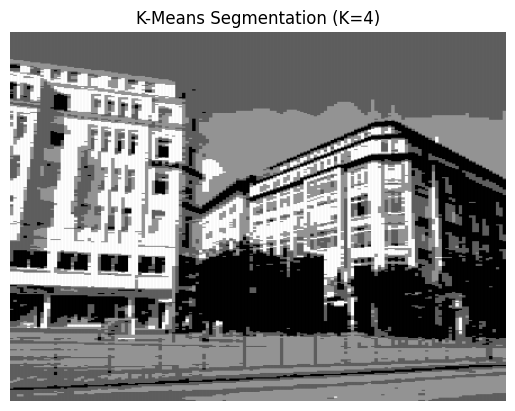
\includegraphics[width=1\textwidth]{k_means.png} 
    \caption{K-means threshold}\label{fig:k_means}
\end{figure}

\subsection{Analysis}
The result in this implementation looks very complex because of many object in the image.
The result show global threshold and k-means segemented the object in the image quite well and adaptive threshold blur the image into continuous object.
The shadow in the global threshold and k-means is completely separate from the building while adaptive threshold delete all the shadow.
Changing the k value showw that the lower the k value will blur the edge especially with lighter color edge.

\section{Feature Extraction}
\subsection{Histogram of Oriented Gradients (HOG)}
HOG focuses on the structure or the shape of an object in the image, it calculates number of direction within each portion in an image
\subsection{Local Binary Pattern (LBP)}
BLP used to describe the texture of an image by comparing each pixel with its neighbors and encodes the local structure into a binary number.
\subsection{Classification}
The implementation of feature extraction use SVM as the classification algorithm and use dataset Fashion-MNIST~\cite{DBLP:journals/corr/abs-1708-07747}.
Codes can be seen below:
\begin{verbatim}
import numpy as np
from tensorflow.keras.datasets import fashion_mnist
from skimage.feature import hog, local_binary_pattern
from sklearn.svm import LinearSVC
from sklearn.preprocessing import StandardScaler
from sklearn.metrics import accuracy_score

# 1. Load Data
(train_images, train_labels), (test_images, 
    test_labels) = fashion_mnist.load_data()
# Subset for speed: 10k for training, 2k for testing
X_tr_raw, y_tr = train_images[:10000], train_labels[:10000]
X_te_raw, y_te = test_images[:2000], test_labels[:2000]

def extract_features(images, mode="combined"):
    features_list = []
    for img in images:
        # HOG
        # Captures the shape/edges
        fd_hog = hog(img, orientations=9, pixels_per_cell=(7, 7), 
                     cells_per_block=(2, 2), visualize=False)
        
        # LBP
        radius = 1
        n_points = 8 * radius
        lbp = local_binary_pattern(img, n_points, 
            radius, method='uniform')
        
        spatial_lbp = []
        cell_size = 7 # 28 / 7 = 4 cells per axis
        for r in range(0, 28, cell_size):
            for c in range(0, 28, cell_size):
                cell = lbp[r:r+cell_size, c:c+cell_size]
                hist, _ = np.histogram(cell, 
                    bins=np.arange(0, n_points + 3), 
                    range=(0, n_points + 2))
                spatial_lbp.extend(
                    hist.astype("float") / 
                    (hist.sum() + 1e-7))
        
        fd_lbp = np.array(spatial_lbp)

        # Selection logic
        if mode == "hog":
            features_list.append(fd_hog)
        elif mode == "lbp":
            features_list.append(fd_lbp)
        else: # combined
            features_list.append(
                np.hstack([fd_hog, fd_lbp]))
            
    return np.array(features_list)

# 2. Extract all three sets
print("Extracting features...")
X_train_hog = extract_features(X_tr_raw, "hog")
X_test_hog = extract_features(X_te_raw, "hog")

X_train_lbp = extract_features(X_tr_raw, "lbp")
X_test_lbp = extract_features(X_te_raw, "lbp")

X_train_comb = extract_features(X_tr_raw, "combined")
X_test_comb = extract_features(X_te_raw, "combined")

# 3. Training & Evaluation Helper
def evaluate(X_train, X_test, y_train, y_test, name):
    scaler = StandardScaler()
    X_train = scaler.fit_transform(X_train)
    X_test = scaler.transform(X_test)
    
    clf = LinearSVC(max_iter=5000, 
        random_state=42, dual=False)
    clf.fit(X_train, y_train)
    acc = accuracy_score(y_test, clf.predict(X_test))
    print(f"{name} Accuracy: {acc*100:.2f}%")

evaluate(X_train_hog, X_test_hog, 
    y_tr, y_te, "HOG Only")
evaluate(X_train_lbp, X_test_lbp, 
    y_tr, y_te, "Spatial LBP Only")
evaluate(X_train_comb, X_test_comb, 
    y_tr, y_te, "HOG + LBP Combined")
\end{verbatim}

Result for this classification can be seen in Table~\ref*{tab:feature_extraction}
\begin{table}[H]
    \centering
    \footnotesize
    \caption{Feature extraction result}\label{tab:feature_extraction}
    \begin{tabular}{@{}lccccc@{}}
        \toprule
        \textbf{Algorithm} & \textbf{Accuracy} \\
        \midrule
        \textbf{HOG}   & \textbf{81.90\%} \\
        \textbf{LBP}   & \textbf{77.55\%} \\
        \textbf{HOG + LBP Combined}     & \textbf{84.05\%} \\
        \bottomrule
    \end{tabular}
\end{table}

\subsection{Analysis}
Classification using feature extraction results shown LBP is the worst method for feature extraction classification of \textbf{77.55\%}.
HOG achieved \textbf{81.90\%} accuracy, while HOG + LBP combined has the highest accuracy of \textbf{84.05\%}.
The combined method achieve such a high accuracy is normal because it has more feature and dimension than only HOG or LBP alone.

\section{Conclusion}
Edge detection has show that sobel has the best depth and shadow edge detection capability while canny capture the most edge.
Segmentation comes with mixed result with k-means threshold offers the better result while global threshold achieve highest contrast between object.

The result of feature extraction classification come with no supprised that combined features achived the highest accuracy using SVM\@.
While LBP has the lowest accuracy because of its limitation using texture which is not a good indication for multi object classification such as Fashion-MNIST.

\printbibliography{}

\end{document}